\documentclass[11pt,a4paper]{article}
\usepackage[T1]{fontenc}
\usepackage{lmodern}
\usepackage[margin=2.5cm]{geometry}
\usepackage{graphicx}
\usepackage{booktabs}
\usepackage{tabularx}
\usepackage{array}
\usepackage{enumitem}
\usepackage{placeins}
\usepackage[dvipsnames]{xcolor}
\usepackage[hidelinks]{hyperref}
\usepackage{caption}
\captionsetup{font=small,labelfont=bf}
\setlist{itemsep=2pt,topsep=4pt}
\setlength{\parskip}{4pt}
\setlength{\parindent}{0pt}
\emergencystretch=3em

% Highlighted placeholder: search for "TODO" and replace before submitting.
\newcommand{\todo}[1]{\textcolor{red}{\textbf{[TODO: #1]}}}

\title{\textbf{CVision}\\[2pt]
  \large Deliverable 1: Problem Definition and Data Foundations\\[2pt]
  \normalsize Track A: Application Development}
\author{Aqsa Ehtesham (24L-3017)\\ M. Shehryar Waheed (24L-3023)}
\date{October 2026}

\begin{document}
\maketitle

\begin{abstract}
\noindent CVision is an explainable CV (resume) evaluation tool for job
seekers: a candidate uploads one PDF and receives an overall quality
score with a category breakdown, specific findings, a role-fit score and
a skill-gap chart. This report covers Phase~1 (the problem statement,
the target audience and the justification for machine learning) and
Phase~2 (data acquisition and preprocessing): collection from two public
Kaggle datasets (2{,}484 resume examples in 24 job categories, and a
40{,}000-posting random sample of 123{,}849 LinkedIn job postings),
cleaning of missing values, duplicates and outliers (leaving 2{,}439 CVs
and 37{,}162 postings), the feature strategy (normalisation, scaling and
encoding), and exploratory data analysis. All code is in the
\texttt{data\_scripts/} folder and the evidence files are in
\texttt{logs/}.
\end{abstract}

\tableofcontents
\newpage


% =====================================================================
\section{Phase 1: Problem Definition}

\subsection{Problem Statement}

Applying for jobs is now largely automated on the employer's side. Many
mid-to-large companies route applications through applicant tracking
systems (ATS) that parse, filter and rank CVs before a human reads them.

Candidates, however, get almost no visibility into this process. A
rejected applicant rarely receives an explanation, and many never learn
whether the problem was weak content, poor formatting, missing skills,
or a layout the ATS could not read. This creates several concrete pain
points:

\begin{itemize}
  \item \textbf{Silent rejection.} Many applicants never hear back, and
  those who do often receive a generic rejection. With no feedback,
  they cannot tell what to change, so they resend the same CV and get
  the same result.
  \item \textbf{Hidden formatting failures.} Tables, multiple columns,
  icons and images can confuse ATS parsers, which may scramble or drop
  entire sections. The candidate sees a clean document, but the system
  reads something broken.
  \item \textbf{Weak, unquantified content.} Many CVs list duties
  (``responsible for sales'') instead of results (``increased sales by
  20\%''). Recruiters skim quickly, and bullets without measurable
  impact are easy to overlook.
  \item \textbf{Unclear skill gaps.} Candidates often do not know which
  skills their target role demands, so they cannot tell what is missing
  from their CV or what to learn next.
  \item \textbf{Unaffordable or untrustworthy help.} Professional CV
  reviews are often expensive, and many free online tools give generic
  advice or push paid upgrades. Students and fresh graduates in
  particular may be unable to afford either option.
\end{itemize}

CVision addresses these problems by turning a single uploaded PDF into
a transparent, explainable evaluation: an overall quality score with a
category breakdown, specific actionable findings, a role-fit score and a
skill-gap chart. The system runs locally on trained models and curated
data, without relying on external AI services. CVision gives feedback to
help a candidate improve a CV; it does not predict or guarantee hiring
outcomes.

\subsection{Target Audience}

\textbf{Primary users}
\begin{itemize}
  \item University students and fresh graduates preparing their first CV
  for internships and entry-level jobs, who typically have no
  professional feedback available. The concrete core user is a
  final-year student applying for a first internship or graduate
  position.
  \item Early-career professionals changing roles or industries who need
  to reposition their experience.
\end{itemize}

\textbf{Secondary users}
\begin{itemize}
  \item University career-services offices and mentors, who could use
  the tool to give consistent first-pass feedback to many students at
  once.
  \item Bootcamp and training institutes, which could use skill-gap
  output to guide learners toward in-demand skills.
  \item Freelancers building profiles for international markets.
\end{itemize}

\subsection{AI Justification}

Rule-based code handles measurable properties well (page length,
section presence, numbers in bullets, and layout features such as tables
or multiple columns detected from the PDF structure), so CVision uses
rules for those. The language-heavy parts need machine learning. Role
fit will be computed as the cosine similarity between sentence-embedding
vectors of the CV and of a job description, and bullet strength by a
classifier trained on labelled bullet points. Both will be compared
against keyword and regular-expression baselines, so that the benefit of
machine learning can be measured rather than assumed.

\begin{itemize}
  \item \textbf{Matching meaning, not keywords.} Rules compare exact
  strings, so ``built predictive models'' would never match a ``machine
  learning'' requirement. Sentence embeddings place similar meanings
  close together, so relevance is captured even when the wording
  differs. This powers the role-fit score.
  \item \textbf{Semantic skill detection.} Whether ``Spark,'' ``R,'' or
  ``Excel'' counts as a skill depends on context, and skills are often
  described rather than named. Comparing CV sentences against a skills
  vocabulary built from job postings, using embeddings, finds skills
  even when the wording varies, where keyword lists give false positives
  or miss variants. This powers the skill-gap chart.
  \item \textbf{Evaluating writing quality.} A regular expression can
  detect a digit but cannot judge whether a bullet communicates real
  impact. A classifier trained on labelled bullet points can assess
  bullet strength more flexibly than a list of banned phrases.
  \item \textbf{Robust section understanding.} CVs have no standard
  format, and headings vary (``Work History,'' ``Career,''
  ``Professional Background''). Semantic models can classify a text
  block as experience, education or projects even under unfamiliar
  headings, while heuristics break.
  \item \textbf{Scalability across roles.} Rule-based systems need
  manual rewriting for each new role or industry. With embeddings,
  adding a role only requires a description or sample postings, with no
  new hand-coded rules.
  \item \textbf{Hybrid design by choice.} Rules keep the quality score
  transparent and auditable, while machine learning supplies semantic
  understanding. Rules alone are too brittle, and a pure black-box model
  would be unexplainable, so combining them gives results users can
  trust and act on.
\end{itemize}

\FloatBarrier
% =====================================================================
\section{Phase 2: Data Acquisition and Preprocessing}

% ---------------------------------------------------------------------
\subsection{Data Collection}
\label{sec:collection}

Two datasets are needed: CV text with a job category (for CV-quality
features, section and writing analysis) and job postings (for the
role-fit score and the skill vocabulary behind the skill-gap chart).
Both were downloaded from Kaggle, and \texttt{collect.py} verifies each
file and records the evidence in \texttt{logs/collection\_log.json}
(source URL, file size, SHA-256 checksum, row and column counts and a UTC
timestamp). With the \texttt{-{}-download} option it fetches missing files
through the Kaggle command-line tool; otherwise the files are placed in
\texttt{data/raw/} manually, and the script prints the exact download
instructions if a file is missing.

\begin{table}[htbp]
  \centering
  \footnotesize
  \begin{tabularx}{\textwidth}{@{}l>{\raggedright\arraybackslash}X>{\raggedright\arraybackslash}X@{}}
    \toprule
    & \textbf{Resume Dataset} & \textbf{LinkedIn Job Postings (2023--2024)} \\
    \midrule
    Kaggle slug & \texttt{snehaanbhawal/resume-dataset} & \texttt{arshkon/linkedin-job-postings} \\
    Origin & Resume examples scraped from livecareer.com by the dataset author & Job postings scraped from LinkedIn by the dataset author \\
    File used & \texttt{Resume.csv} & \texttt{postings.csv} \\
    Size & 56.27 MB & 516.84 MB \\
    Rows $\times$ columns & 2{,}484 $\times$ 4 & 123{,}849 $\times$ 31 \\
    Main columns & ID, Resume\_str, Resume\_html, Category & job\_id, title, description, skills\_desc, formatted\_experience\_level, formatted\_work\_type, salary fields, views, applies, \dots \\
    Used for & CV-quality features, category analysis & Role-fit scoring, skill vocabulary, skill-gap chart \\
    SHA-256 (first 16 characters) & \texttt{816a7cd985a9a41e} & \texttt{de33f27c8d1b2260} \\
    Collected & 17 Oct 2026 (UTC) & 17 Oct 2026 (UTC) \\
    License & CC0: Public Domain & CC BY-SA 4.0 \\
    \bottomrule
  \end{tabularx}
  \caption{Datasets used, as recorded in \texttt{collection\_log.json}.}
  \label{tab:datasets}
\end{table}

Table~\ref{tab:datasets} summarises both sources. The full dataset
pages are listed in the references \cite{kaggle_resume,kaggle_jobs}. The
raw files are not stored in the GitHub repository because of their size
(the postings file alone is about 517~MB); the checksums in the log allow
anyone to confirm that they have downloaded identical files. Only the
columns needed by the project are read from the postings file, and a
random sample of 40{,}000 postings (seed 42) is used to keep processing
fast.

% ---------------------------------------------------------------------
\subsection{Data Cleaning}
\label{sec:cleaning}

Cleaning is implemented in \texttt{clean.py} and covers the three
required problems: missing values, duplicates and outliers. Every
removed row is written to an audit file (\texttt{resumes\_audit.csv},
\texttt{jobs\_audit.csv}) with the reason for its removal, so no record
disappears silently, and the totals are stored in
\texttt{logs/cleaning\_report.json}.

\textbf{Text cleaning (both datasets).} HTML tags and entities left over
from web scraping are removed, Unicode is normalised (NFKC), decorative
symbols are dropped and whitespace is collapsed.

\textbf{Missing values.}
\begin{itemize}
  \item \emph{CVs:} no raw column contains nulls (Figure~\ref{fig:missing}),
  but a CV whose text is empty after cleaning, or whose category is
  missing, cannot be used and is dropped. One CV (a Business-Development
  CV with 0 words) was removed this way. Category labels are stripped
  and put in title case.
  \item \emph{Job postings:} a posting without a title or description
  is dropped (3 postings in the sample). Missing work type, experience
  level, company name and location are filled with ``Unknown'', a
  missing \texttt{remote\_allowed} is set to 0, and the very sparse
  \texttt{skills\_desc} column is kept with a binary
  \texttt{has\_skills\_desc} flag. Missing \texttt{views} and
  \texttt{applies} are median-imputed and flagged.
\end{itemize}

\textbf{Duplicates.}
\begin{itemize}
  \item \emph{CVs:} exact duplicates of the cleaned text are removed
  (2 found), followed by near-duplicates detected through an MD5 hash of
  the normalised (lower-case, punctuation-free) text (none found).
  \item \emph{Job postings:} duplicate job IDs are removed (none found),
  followed by reposts, defined as the same title, company and normalised
  description (2{,}560 found, 6.4\% of the sample).
\end{itemize}

\textbf{Outliers.}
\begin{itemize}
  \item \emph{Length (both datasets):} documents shorter than a minimum
  (50 words for CVs, 30 for postings) are not real CVs or postings, and
  documents above the upper fence $Q_3 + 3.0 \times \mathrm{IQR}$ are
  treated as extreme outliers. The fences are 1{,}778 words for CVs and
  1{,}896 words for postings. A factor of 3.0 (instead of the usual 1.5)
  removes only genuinely extreme documents.
  \item \emph{Salary:} pay is converted to a yearly figure (hourly
  $\times$ 2{,}080, weekly $\times$ 52, biweekly $\times$ 26, monthly
  $\times$ 12), non-positive values and values above 5{,}000{,}000 are
  treated as missing, and the remaining values are winsorised to the 1st
  and 99th percentiles (92 to 297{,}157). Because the lower bound is
  implausibly low, a few erroneous yearly values remain; salary is
  therefore used only as a weak, optional feature.
\end{itemize}

\begin{table}[htbp]
  \centering
  \small
  \begin{tabular}{@{}lrr@{}}
    \toprule
    Step & CVs & Job postings \\
    \midrule
    Raw rows & 2{,}484 & 123{,}849 \\
    Random sample (seed 42) & --- & 40{,}000 \\
    Missing or empty (title/description/text) & 1 & 3 \\
    Exact or ID duplicates & 2 & 0 \\
    Near-duplicates / reposts & 0 & 2{,}560 \\
    Too short (CV $<$ 50 words, posting $<$ 30 words) & 0 & 207 \\
    Too long (above IQR fence) & 42 & 68 \\
    \midrule
    \textbf{Rows kept} & \textbf{2{,}439 (98.2\%)} & \textbf{37{,}162 (92.9\% of sample)} \\
    \bottomrule
  \end{tabular}
  \caption{Rows removed at each cleaning step
  (from \texttt{cleaning\_report.json}).}
  \label{tab:cleaning}
\end{table}

Table~\ref{tab:cleaning} gives the number of rows removed at every
step. The figures in Section~\ref{sec:eda} (missing values, length
before and after cleaning) show the effect of these steps.

% ---------------------------------------------------------------------
\subsection{Feature Strategy}
\label{sec:features}

Feature engineering is implemented in \texttt{features.py}. It covers
normalisation, scaling and encoding, and all statistics are learned on
the training split only to avoid data leakage.

\textbf{Normalisation.} Besides the light cleaning above, an aggressive
normalisation is used for text models: lower-casing, removal of all
characters except letters, digits, ``+'' and ``\#'' (so that terms such
as C++ and C\# survive) and collapsing of whitespace.

\textbf{CV features (hand-crafted and explainable).} Thirteen numeric
features are computed for each CV; they feed the transparent part of the
quality score (Table~\ref{tab:cvfeatures}).

\begin{table}[htbp]
  \centering
  \footnotesize
  \begin{tabularx}{\textwidth}{@{}>{\ttfamily}l>{\raggedright\arraybackslash}X@{}}
    \toprule
    Feature & Definition \\
    \midrule
    word\_count, sentence\_count & Tokens and sentences in the CV \\
    avg\_sentence\_len, avg\_word\_len & Mean words per sentence, mean characters per word \\
    lexical\_diversity & Unique words divided by words, over the first 300 tokens (length-robust) \\
    metric\_number\_count & Numbers in the CV that are not years \\
    percent\_count & Number of ``\%'' signs \\
    numbers\_per\_100\_words & Non-year numbers per 100 words \\
    quantified\_sentence\_ratio & Share of sentences containing a non-year number \\
    action\_verb\_count, action\_verbs\_per\_100\_words & Matches against a list of 49 achievement verbs (``led'', ``increased'', \dots), raw and per 100 words \\
    section\_count & Number of the 7 section types (summary, experience, education, skills, projects, certifications, awards) whose keywords occur in the text \\
    skill\_count & Number of skills from a 70-skill vocabulary found in the CV \\
    \bottomrule
  \end{tabularx}
  \caption{Numeric features computed for each CV.}
  \label{tab:cvfeatures}
\end{table}

\textbf{Job features.} For postings, the numeric features are the
description word count, title word count, length of the skills text,
number of vocabulary skills found in the title, description and skills
text, yearly salary, views and applies. The 70-skill vocabulary is
hand-written (programming, data, cloud, business and soft skills) and is
matched by exact keywords; it serves only as a baseline for the skill
analysis.

\textbf{Text encoding.} CV text is converted into TF-IDF vectors
(unigrams and bigrams, English stop words removed, at least 3 documents
per term, sub-linear term frequency, vocabulary limited to 5{,}000
terms). The vectoriser is fitted on the training CVs only.

\textbf{Scaling.} Numeric features are scaled in two steps. First,
$\log(1+x)$ is applied automatically to every feature whose
training-set skewness is greater than 1.0, which compresses long right
tails. Second, all numeric features are standardised to zero mean and
unit variance with a scaler fitted on the training split. The $\log(1+x)$
step was applied to \texttt{avg\_sentence\_len},
\texttt{metric\_number\_count}, \texttt{percent\_count},
\texttt{numbers\_per\_100\_words}, \texttt{quantified\_sentence\_ratio}
and \texttt{action\_verb\_count} for CVs, and to title length, skills
text length, skill count, yearly salary, views and applies for postings.
Figure~\ref{fig:scaling} shows the effect on one feature.

\textbf{Encoding.}
\begin{itemize}
  \item The 24 CV categories are encoded as integers 0--23
  (label encoding) and the mapping is stored in
  \texttt{logs/feature\_report.json}.
  \item Job work type (7 values) and experience level (7 values,
  including ``unknown'') are one-hot encoded into 14 columns.
  \item Binary indicators are kept for \texttt{remote\_allowed},
  \texttt{has\_skills\_desc} and \texttt{salary\_missing}; missing
  yearly salaries are filled with the median.
\end{itemize}

\textbf{Train/test split.} The 2{,}439 CVs are split 80/20 with
stratification by category (random seed 42) into 1{,}951 training and
488 test CVs. No separate validation split has been created yet.

\FloatBarrier
% ---------------------------------------------------------------------
\subsection{Exploratory Data Analysis}
\label{sec:eda}

This section interprets the exploratory charts produced by
\texttt{eda.py}. Two datasets are analysed: the Kaggle \emph{Resume
Dataset} (2{,}484 raw CVs, 24 job categories) and a sample of 40{,}000
postings drawn from the Kaggle \emph{LinkedIn Job Postings} dataset
(123{,}849 raw postings). Cleaning reduced them to 2{,}439 CVs and
37{,}162 postings, respectively.

% ---------------------------------------------------------------
\subsubsection{CV dataset}

\begin{figure}[htbp]
  \centering
  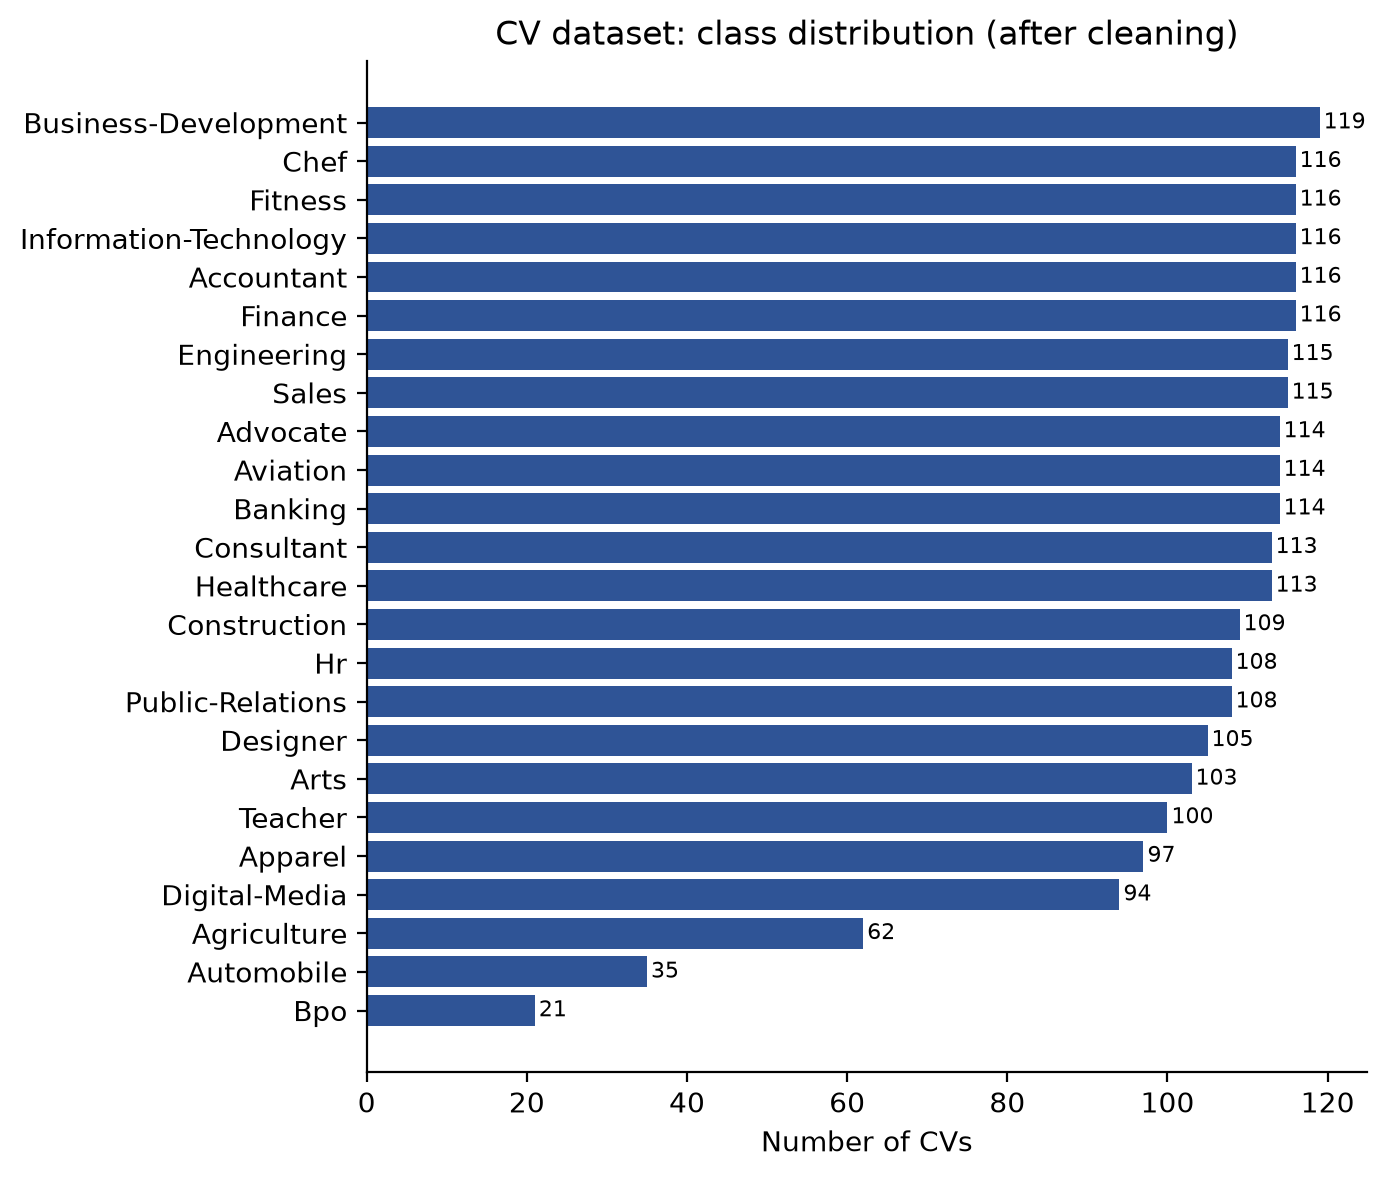
\includegraphics[width=0.85\textwidth]{figures/fig01_cv_category_distribution.png}
  \caption{Number of CVs per job category after cleaning.}
  \label{fig:cv_classes}
\end{figure}

Figure~\ref{fig:cv_classes} shows the number of CVs in each of the 24
job categories after cleaning. Twenty-one categories are well balanced,
with between 94 and 119 CVs each. Three categories are clearly
under-represented: Agriculture (62), Automobile (35) and BPO (21),
which gives a largest-to-smallest class ratio of 5.67 (5.45 before cleaning, with 120 CVs in the largest and 22 in the smallest category, so cleaning did not change the class structure). A model trained
on this distribution would see far fewer examples of these categories
and could perform worse on them, and any per-category statistic for BPO
or Automobile rests on very few CVs. We therefore use a stratified
train/test split (1{,}951 / 488 CVs), report macro-averaged metrics in
addition to accuracy, and plan to apply class weights during training.

\begin{figure}[htbp]
  \centering
  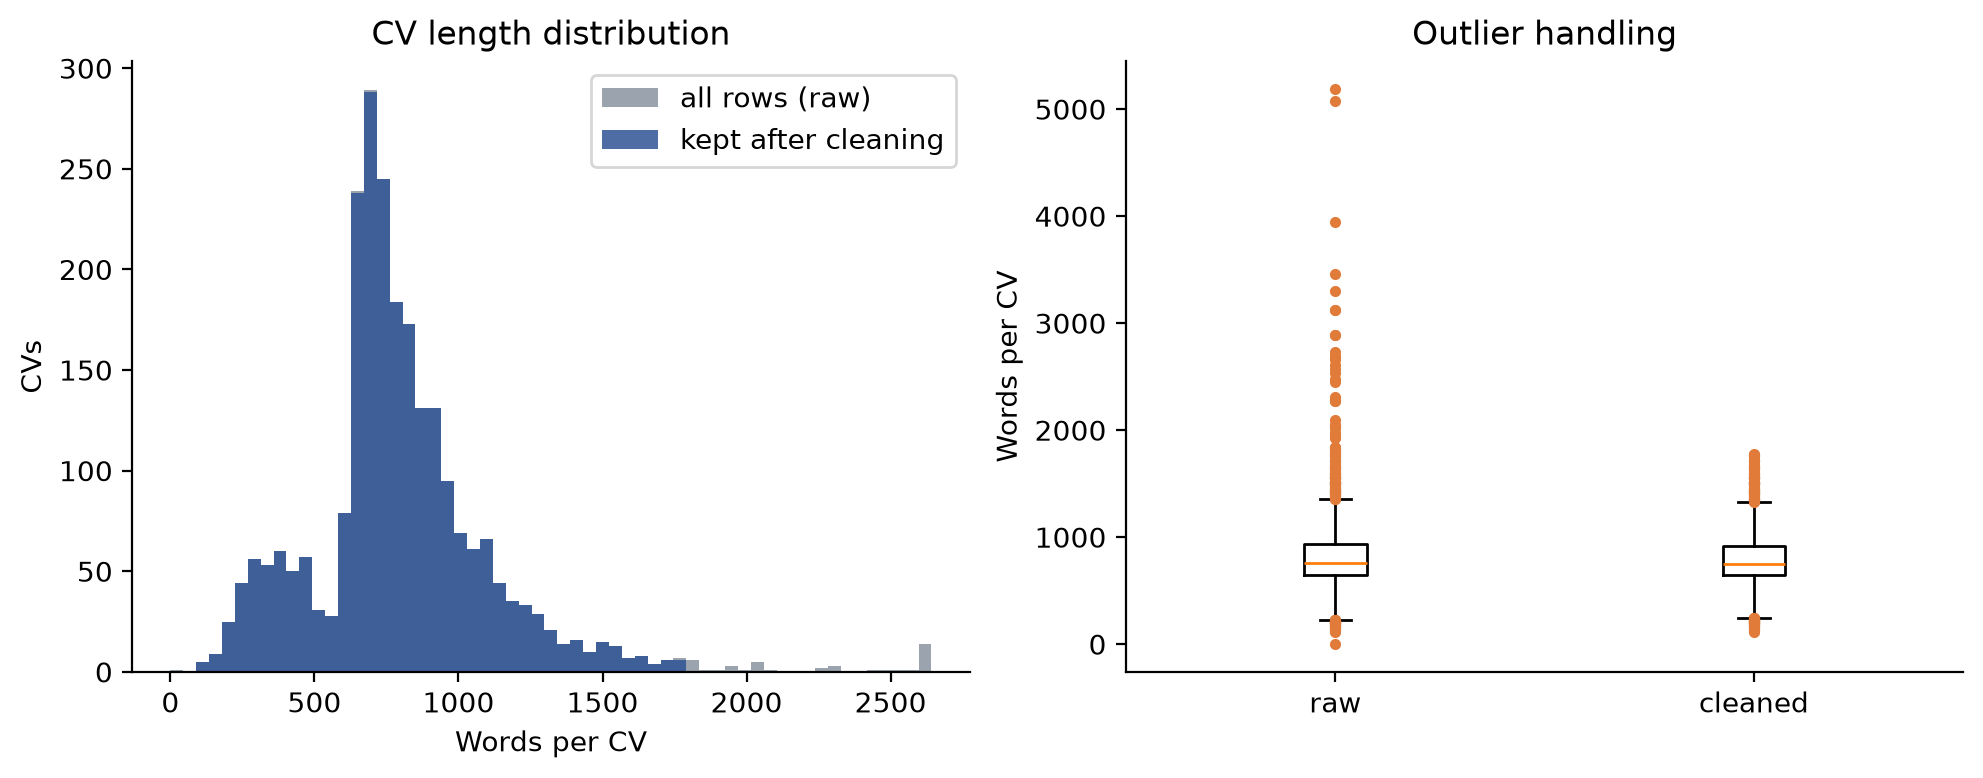
\includegraphics[width=\textwidth]{figures/fig02_cv_length_before_after.png}
  \caption{CV length in words, before and after outlier handling
  (left: histogram, right: box plot). In the histogram, values above
  the 99.5th percentile of the raw data ($\approx$2{,}640 words) are
  clipped into the last bin.}
  \label{fig:cv_length}
\end{figure}

Figure~\ref{fig:cv_length} compares CV length before and after
cleaning. The cleaned distribution has a median of 751 words, a main
peak between roughly 650 and 800 words, a smaller secondary peak
around 250--450 words, and a long right tail. In the raw data the
longest CVs reach about 5{,}200 words. The outlier rule removed CVs
above the upper fence $Q_3 + 3.0 \times \mathrm{IQR} = 1{,}778$ words
(42 CVs, 1.7\% of the data); the minimum-length rule (50 words) removed
none. The box plot shows that the median and the interquartile range
are essentially unchanged by cleaning, so the extreme values were
removed without shifting the bulk of the data. We keep the secondary
peak of short CVs because it appears to reflect a genuine, concise CV
style rather than an error, and CVision's length rule must handle it.
Overall, cleaning took the dataset from 2{,}484 to 2{,}439 CVs (42
length outliers, 2 exact duplicates and 1 missing record removed),
retaining 98.2\%.

\begin{figure}[htbp]
  \centering
  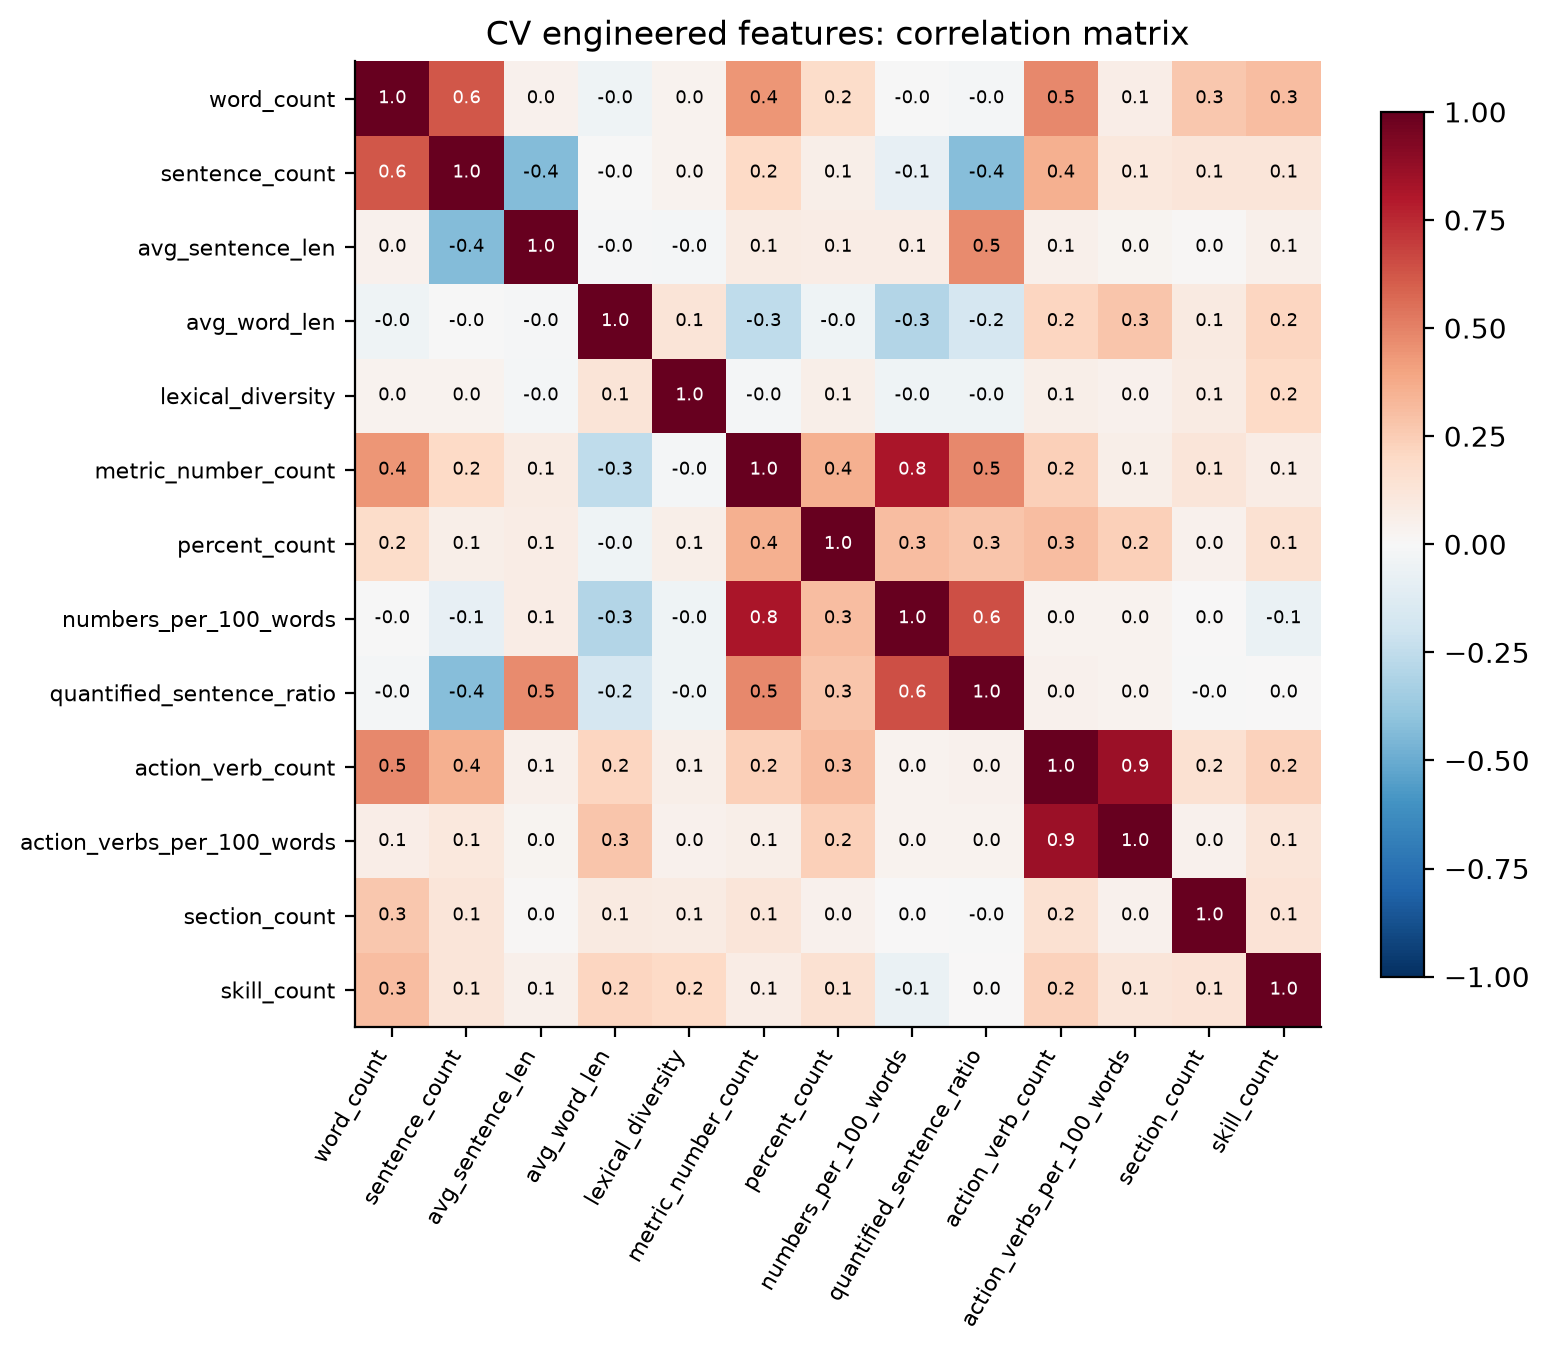
\includegraphics[width=0.85\textwidth]{figures/fig03_cv_feature_correlation.png}
  \caption{Correlation matrix of the engineered CV features.}
  \label{fig:cv_corr}
\end{figure}

Figure~\ref{fig:cv_corr} shows the pairwise correlations between the
13 engineered CV features. Three groups of strongly related features
stand out: the action-verb count and its per-100-word version
($r \approx 0.9$), the metric-number count and numbers per 100 words
($r \approx 0.8$), and word count with sentence count
($r \approx 0.6$). Raw counts also correlate with CV length (for
example, action-verb count with word count, $r \approx 0.5$), whereas
the per-100-word versions do not (about 0.1 and 0.0). Most other pairs
are weak, and \texttt{section\_count}, \texttt{skill\_count} and
\texttt{lexical\_diversity} are only weakly related to everything
else ($|r| \le 0.3$), so they carry largely independent information. Note that
\texttt{section\_count} is a keyword-presence heuristic (the number of
section keywords such as ``experience'' or ``education'' found anywhere
in the text), not a true section detector, which explains its weak
correlations; real section understanding is left to the models of later
phases.
The strong pairs are partly redundant. For linear models we will keep
the length-independent density features
(\texttt{numbers\_per\_100\_words}, \texttt{action\_verbs\_per\_100\_words})
and drop or regularise their raw-count counterparts to avoid
multicollinearity; tree-based models are not affected by this.

\begin{figure}[htbp]
  \centering
  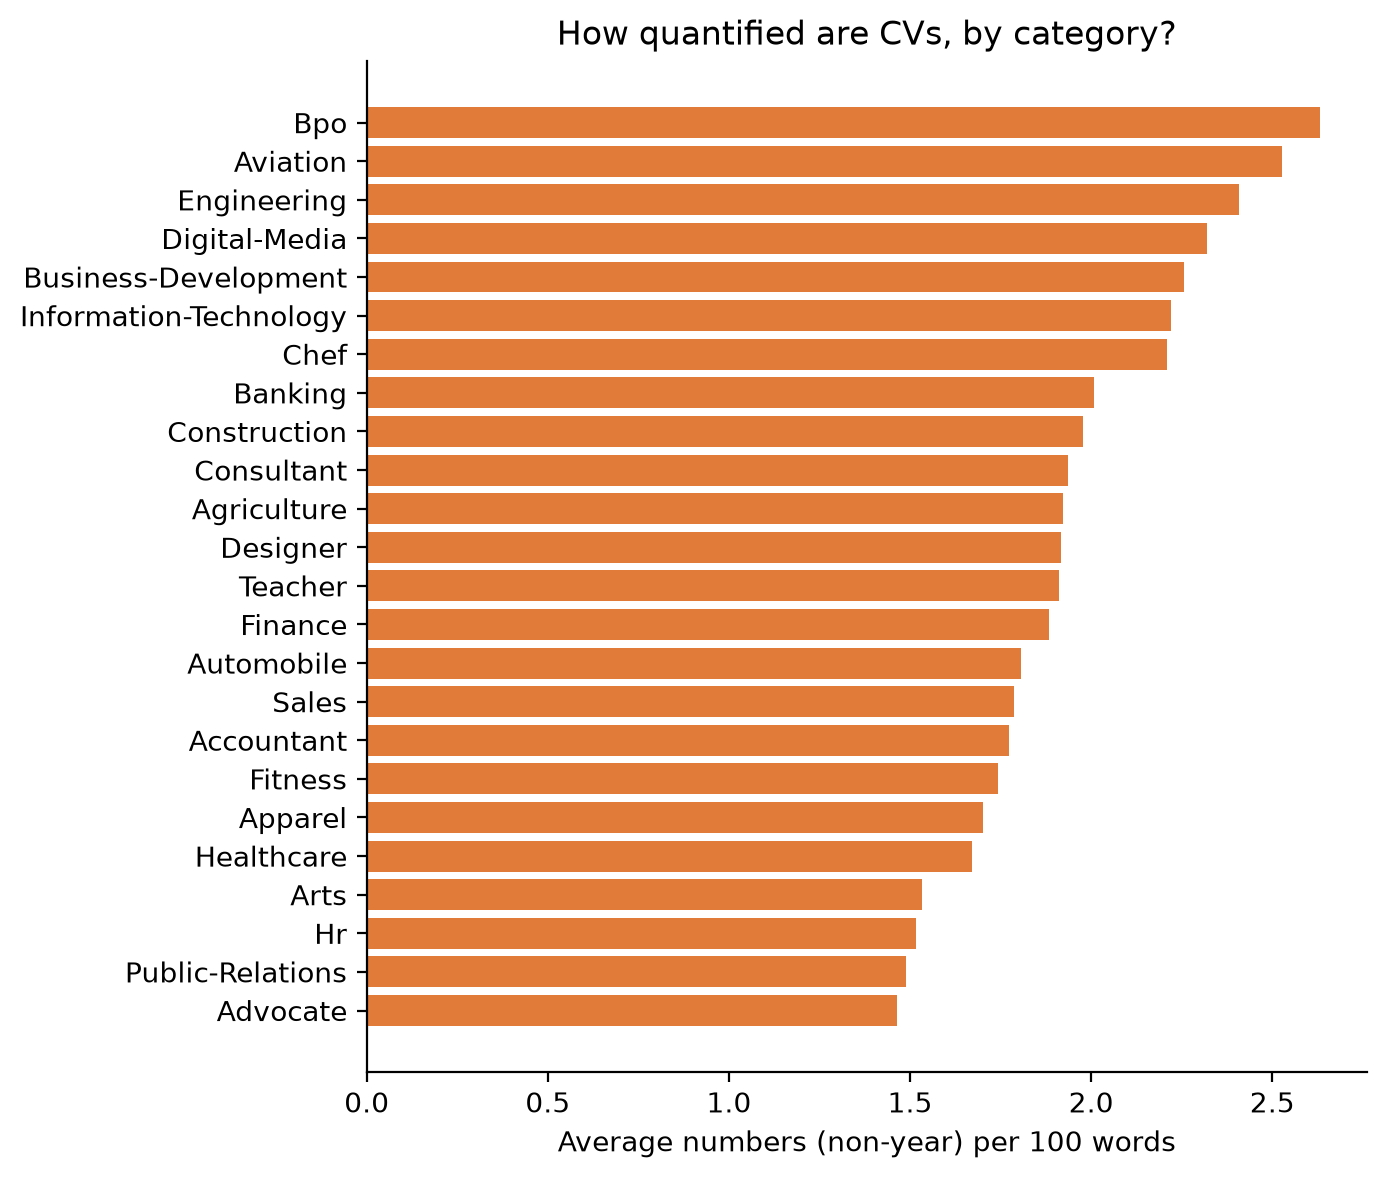
\includegraphics[width=0.85\textwidth]{figures/fig04_cv_quantification_by_category.png}
  \caption{Average number of non-year numbers per 100 words, by CV
  category.}
  \label{fig:cv_quant}
\end{figure}

Figure~\ref{fig:cv_quant} shows how quantified CVs are in each
category, measured as the average number of non-year numbers per 100
words. Values range from about 1.5 (Advocate) to about 2.6 (BPO).
Technical and operational categories such as Aviation, Engineering,
Digital-Media and Information-Technology sit near the top, while
people- and service-oriented categories such as Advocate, Public
Relations, HR and Arts sit near the bottom. BPO is the highest, but it
has only 21 CVs, so its value is the least reliable. This matters for
CVision's ``quantified impact'' check: a single global threshold would
systematically penalise categories in which numbers are naturally less
common. The rule should therefore be calibrated per category or
expressed relative to the target role.

% ---------------------------------------------------------------
\subsubsection{Job postings dataset}

\begin{figure}[htbp]
  \centering
  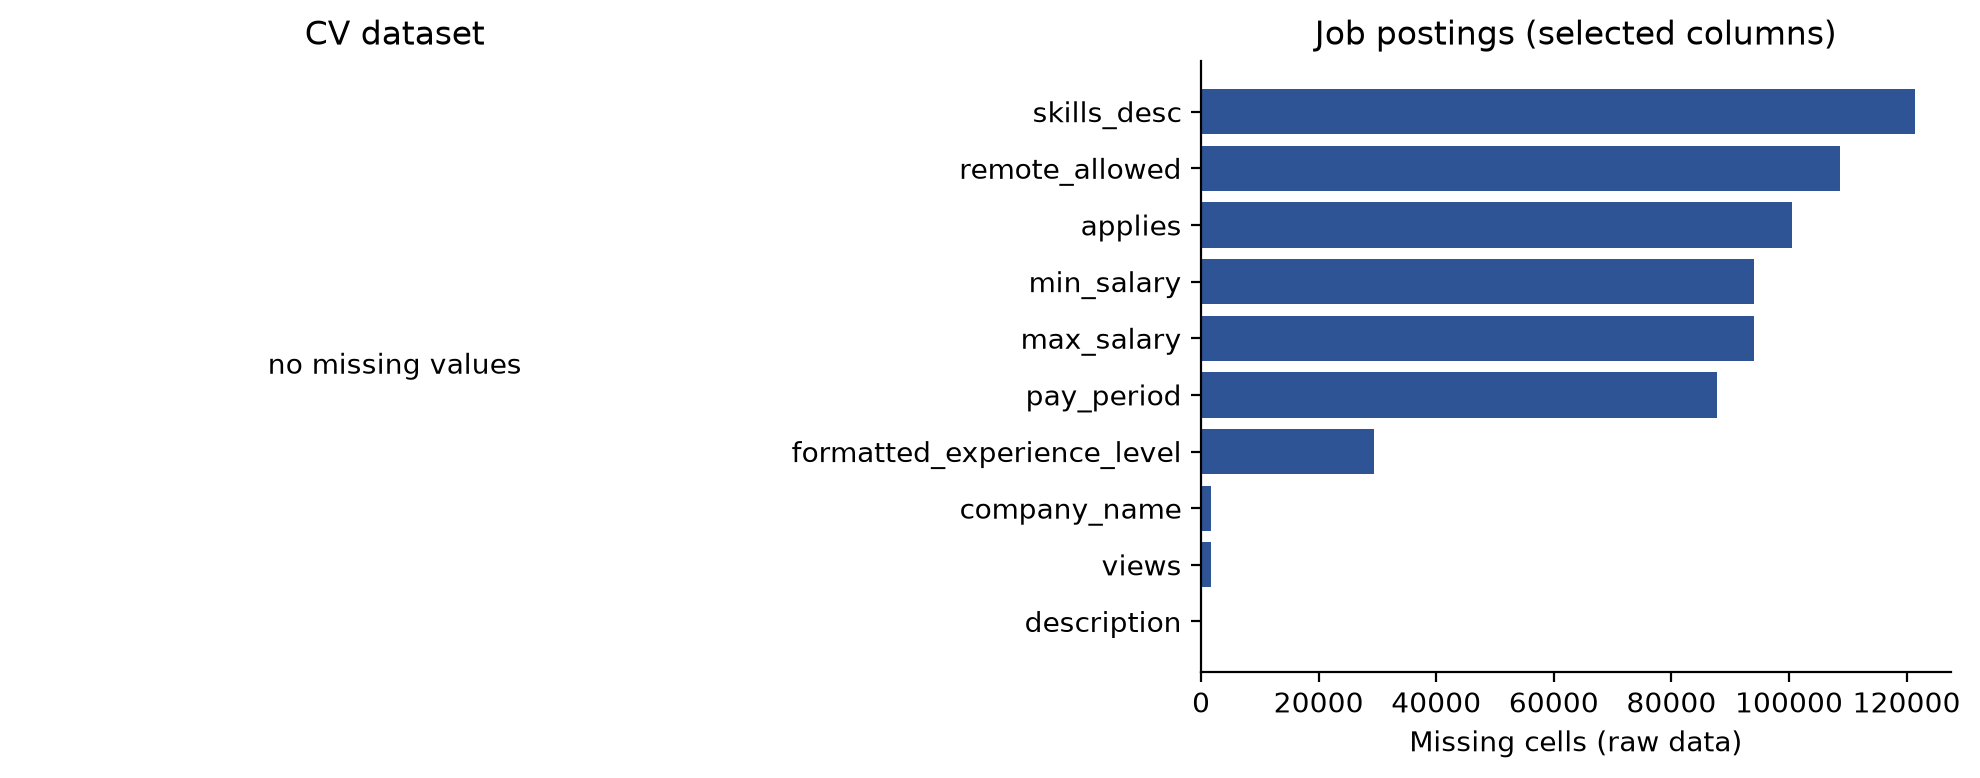
\includegraphics[width=\textwidth]{figures/fig05_missing_values.png}
  \caption{Missing values per column in the raw data.}
  \label{fig:missing}
\end{figure}

Figure~\ref{fig:missing} summarises missing data. The CV dataset has
no missing values in any of its four columns. The job postings are
much less complete: \texttt{skills\_desc} is empty for 98.0\% of
postings (121{,}410 of 123{,}849), \texttt{remote\_allowed} for 87.7\%,
\texttt{applies} for 81.2\%, both salary bounds for 75.9\%,
\texttt{pay\_period} for 70.9\%, and
\texttt{formatted\_experience\_level} for 23.7\%. Company name and
views are missing for about 1.4\% each, and only 7 postings lack a
description. Because \texttt{skills\_desc} is almost always empty, the
skill vocabulary must be derived from the free-text description rather
than from this column. Salary is too sparse to serve as a reliable
target, so we treat it as an optional feature (winsorised to
92--297{,}157; the very low lower bound shows that a few implausible
yearly values remain, which we did not filter further), and missing experience levels are encoded as an explicit
``unknown'' category. Missing \texttt{views} and \texttt{applies}
values are median-imputed and flagged, and a missing
\texttt{remote\_allowed} is encoded as 0 (not stated as remote); since
these fields are so sparse, they will be treated as weak features. Only
postings without a title or description, which cannot be used at all,
are dropped (3 in the 40{,}000-posting sample).

\begin{figure}[htbp]
  \centering
  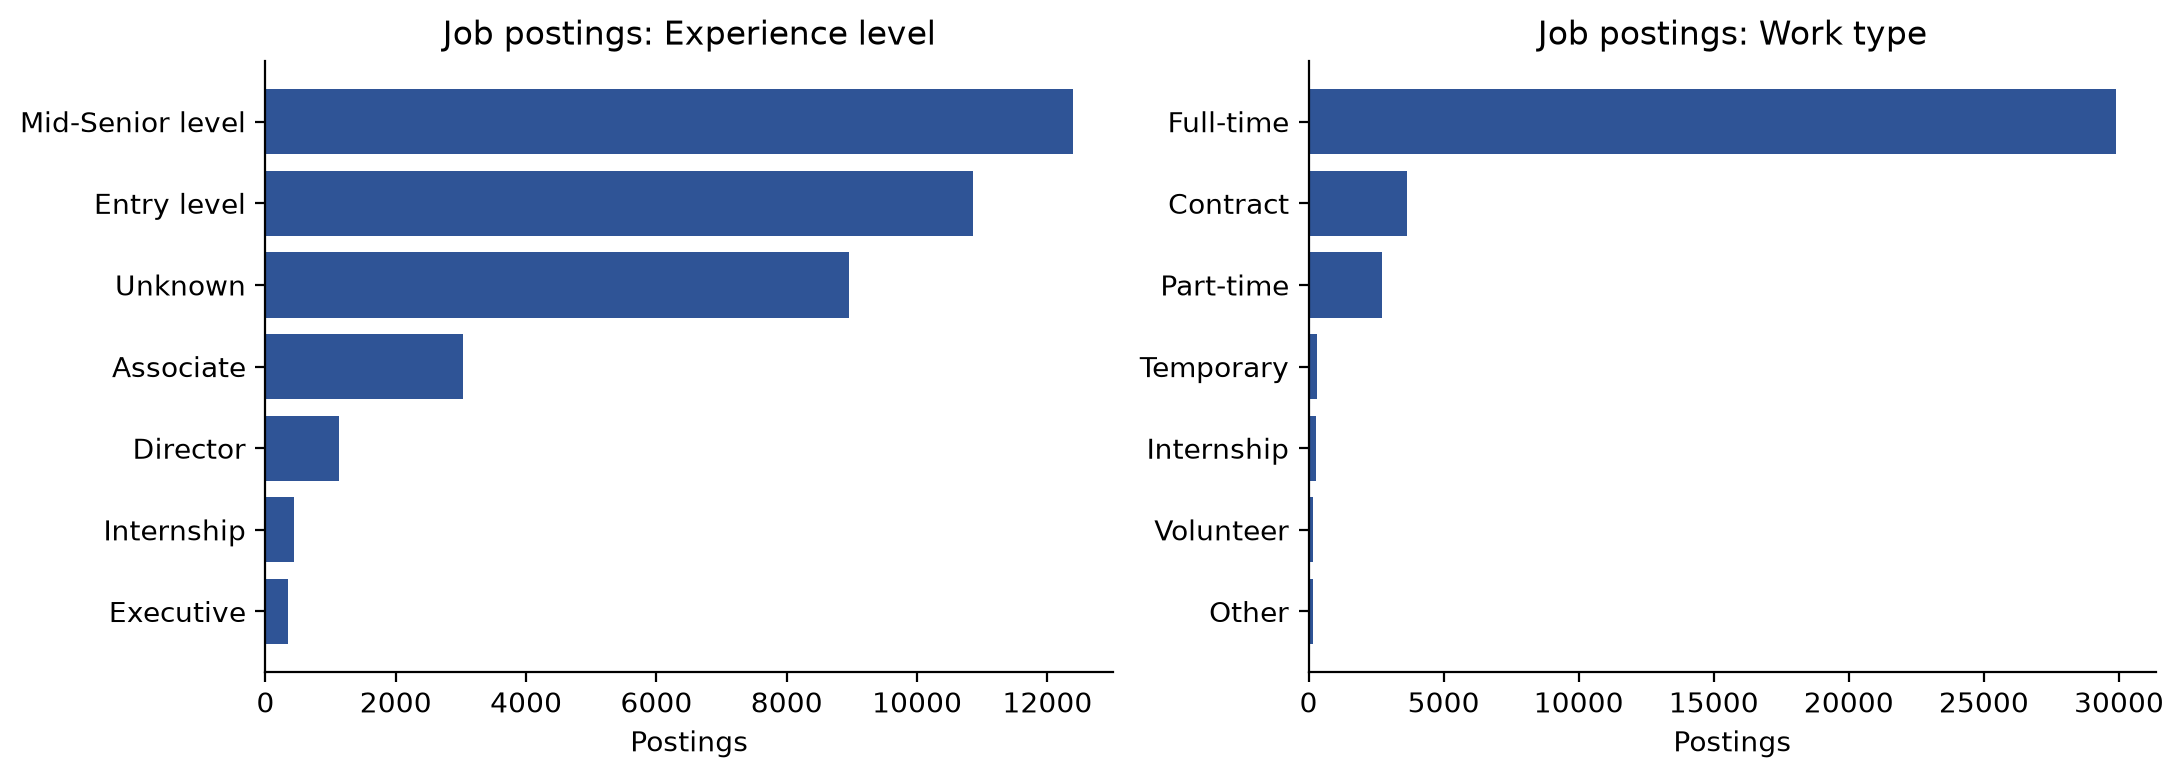
\includegraphics[width=\textwidth]{figures/fig06_job_categorical_distributions.png}
  \caption{Distribution of experience level (left) and work type
  (right) in the cleaned postings.}
  \label{fig:job_cat}
\end{figure}

Figure~\ref{fig:job_cat} shows the categorical structure of the
cleaned postings. Mid-Senior level is the largest experience level
(about 12{,}400 postings), followed by Entry level (about 10{,}900,
roughly 29\%) and ``Unknown'' (about 9{,}000, which corresponds to the
missing values above). Associate, Director, Internship and Executive
postings are much rarer, and internships account for only about 1\% of
the data. Work type is heavily dominated by Full-time (about 29{,}900
postings, roughly 80\%), followed by Contract and Part-time, with
Temporary, Internship, Volunteer and Other each under 1\%. The
sizeable Entry-level share is encouraging for CVision's primary users
(students and fresh graduates), but internship-specific postings are
scarce, so role-fit results for internships will be less well
supported. The very small work-type categories will be grouped or
interpreted with caution when used as one-hot features.

\begin{figure}[htbp]
  \centering
  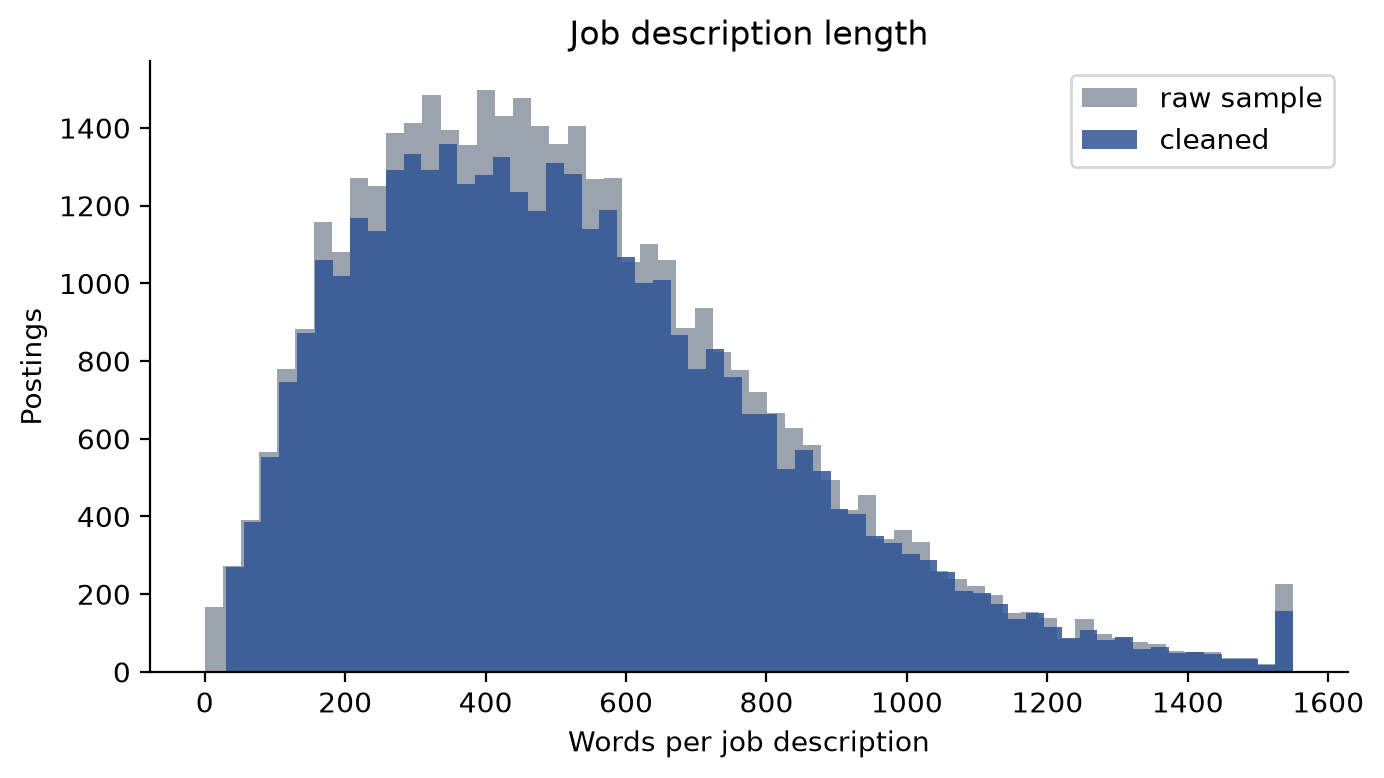
\includegraphics[width=0.85\textwidth]{figures/fig07_job_description_length.png}
  \caption{Job description length in words, raw sample versus cleaned
  data. Values above the 99.5th percentile of the raw sample
  ($\approx$1{,}550 words) are clipped into the last bin.}
  \label{fig:job_length}
\end{figure}

Figure~\ref{fig:job_length} shows the length of job descriptions. The
cleaned distribution is right-skewed with a median of 482 words and
most postings between about 200 and 800 words. Cleaning removed 2{,}560
duplicate reposts (6.4\% of the 40{,}000-posting sample), 207 postings
shorter than 30 words, 68 longer than 1{,}896 words and 3 with a missing title or
description, retaining 37{,}162 postings (92.9\%). The grey-versus-blue
comparison shows that duplicate removal reduced the counts across the
whole range, while the very short postings, which carry almost no skill
information, disappear from the left edge. Postings (median 482 words)
are shorter than CVs (median 751 words), and both are long enough that
embedding models with a limited input length would truncate them. Texts
will therefore need to be split into chunks, such as by section, before
embedding.

% ---------------------------------------------------------------
\subsubsection{Skill demand versus skill supply}

\begin{figure}[htbp]
  \centering
  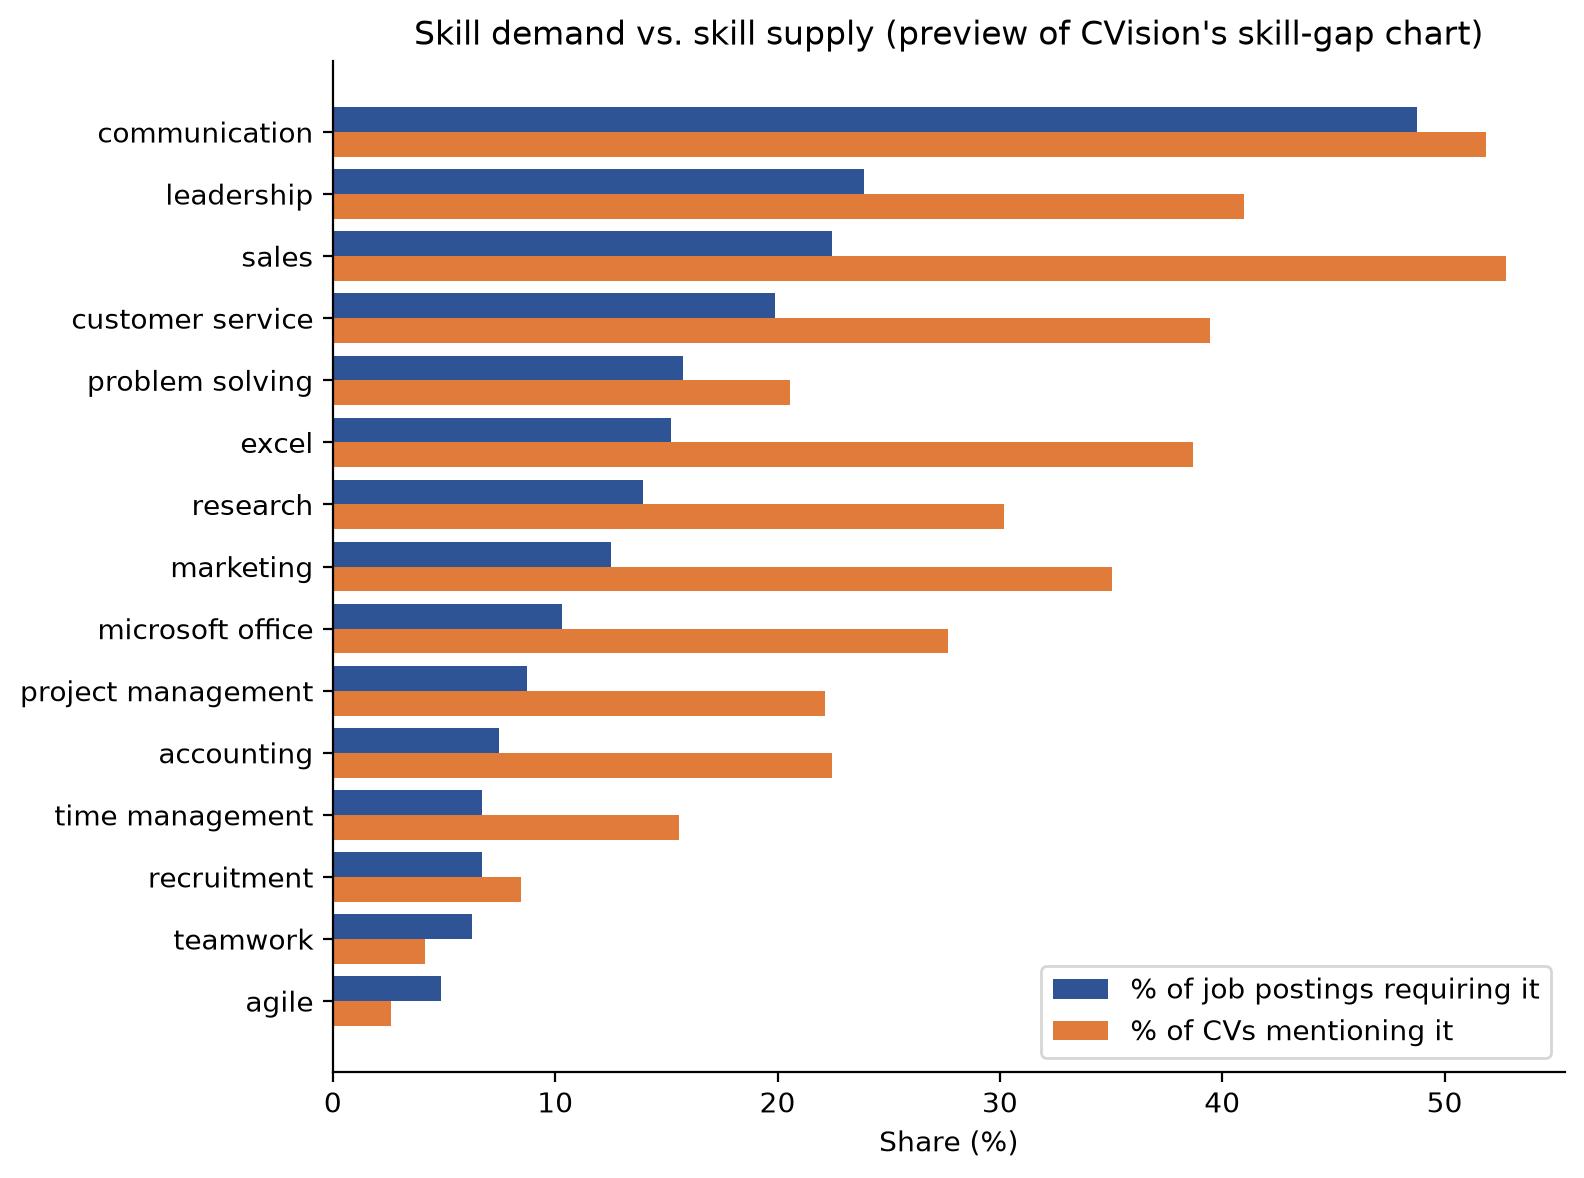
\includegraphics[width=0.85\textwidth]{figures/fig08_skill_gap_preview.png}
  \caption{Share of job postings requiring each skill versus share of
  CVs mentioning it (preview of CVision's skill-gap chart).}
  \label{fig:skill_gap}
\end{figure}

Figure~\ref{fig:skill_gap} previews the skill-gap chart by comparing
the share of postings that require a skill with the share of CVs that
mention it, using exact keyword matching over a hand-written 70-skill vocabulary;
the chart shows the 15 skills with the highest posting share.
Communication is the most requested skill (48.7\% of postings) and is
mentioned about as often on CVs (51.9\%). For most other skills CVs
mention them far more often than postings require them: sales
(about 53\% of CVs versus 22\%), excel (39\% versus 15\%), marketing
(35\% versus 13\%), customer service (39\% versus 20\%) and leadership
(41\% versus 24\%). Only a few skills are demanded more than supplied,
notably agile (4.9\% versus 2.6\%) and teamwork (6.3\% versus 4.1\%),
and among technical skills Python (3.7\% versus 1.6\%), AWS, Azure,
Docker, Kubernetes and machine learning. Six vocabulary skills
(TypeScript, deep learning, PyTorch, NLP, Kubernetes and Django) do not
appear in any CV. These results should be read with care. The CV
dataset spans 24 mostly non-technical occupations and appears to
under-represent modern technical profiles, and CVs are longer and more
skill-dense than postings, so the dataset-level gap is not a true
candidate-level gap. The final CVision chart will instead compare an
individual CV with the postings of the chosen target role. This preview
also uses exact keyword matching, which cannot recognise paraphrased
skills, which motivates embedding-based semantic matching in later
phases. We also plan to add more technical CVs to
test the technical-role case.

% ---------------------------------------------------------------
\subsubsection{Effect of scaling}

\begin{figure}[htbp]
  \centering
  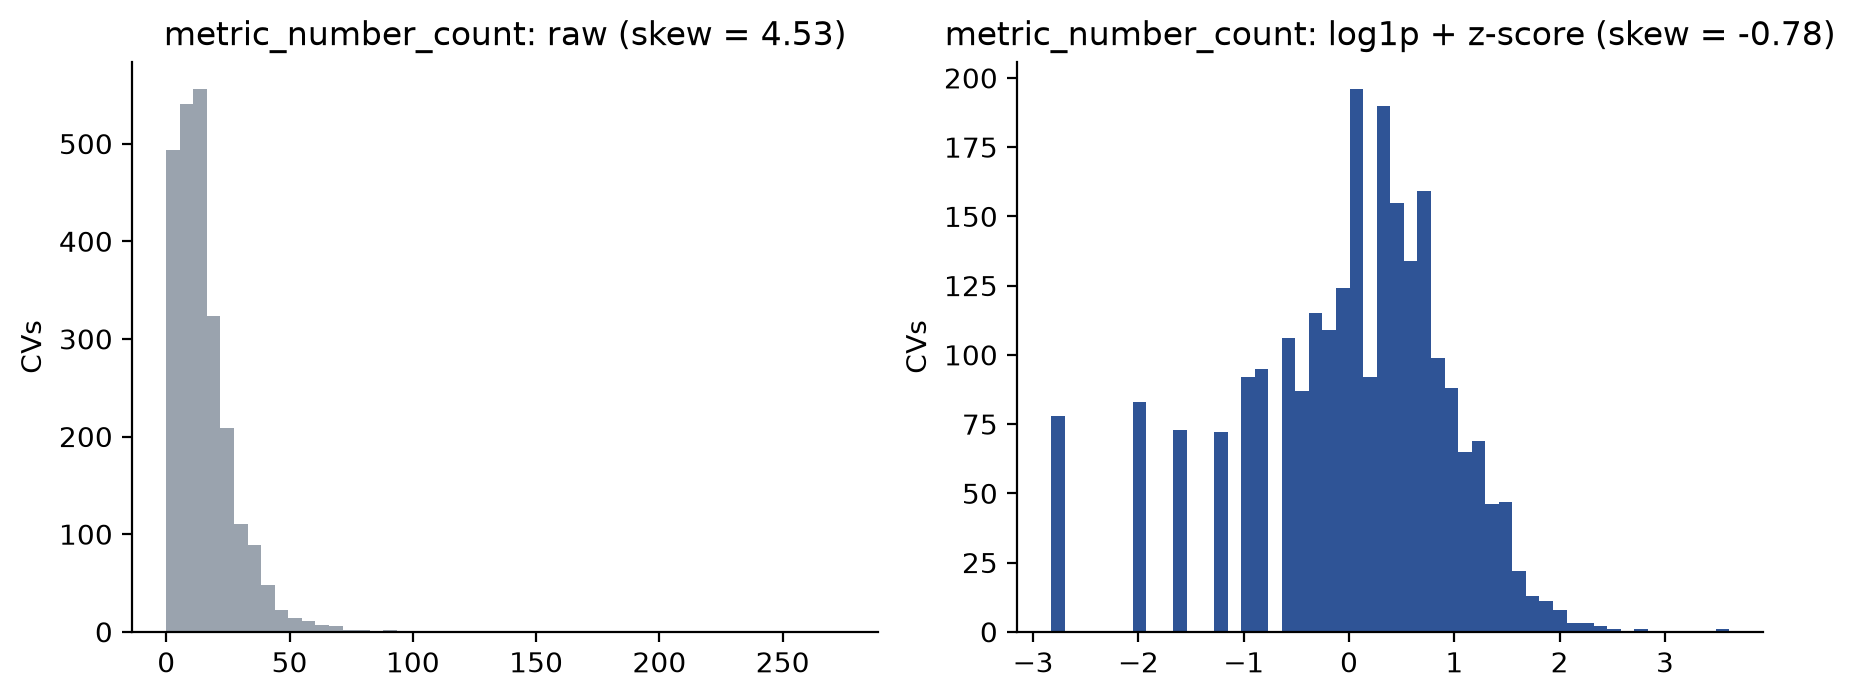
\includegraphics[width=\textwidth]{figures/fig09_scaling_effect.png}
  \caption{Distribution of \texttt{metric\_number\_count} before
  (left) and after (right) the $\log(1+x)$ transform and
  standardisation.}
  \label{fig:scaling}
\end{figure}

Figure~\ref{fig:scaling} shows the effect of the scaling pipeline on
\texttt{metric\_number\_count}, the number of non-year numbers in a CV.
The raw distribution is strongly right-skewed (skewness 4.53): most CVs
contain fewer than about 30 such numbers, while a few exceed 100 and
the largest reaches roughly 270. Applying $\log(1+x)$ followed by
z-score standardisation compresses this tail and gives a far more
symmetric distribution (skewness $-0.78$) with zero mean and unit
variance, spanning roughly $-2.9$ to $3.6$. The isolated bars on the
left are an artefact of integer counts, because $\log(1+x)$ of the
smallest values (0, 1, 2, \dots) is well separated; the leftmost bar
most likely corresponds to CVs containing no numbers at all. The
transform slightly over-corrects, leaving a mild left skew, but this is a
large improvement for distance-based and regularised models, which
would otherwise be dominated by a few extreme CVs. The pipeline applies
$\log(1+x)$ automatically, and only to features whose training-set
skewness exceeds 1.0: \texttt{avg\_sentence\_len},
\texttt{metric\_number\_count}, \texttt{percent\_count},
\texttt{numbers\_per\_100\_words}, \texttt{quantified\_sentence\_ratio}
and \texttt{action\_verb\_count} for CVs, and title length, skills text
length, skill count, yearly salary, views and applies for postings.
Less skewed features such as \texttt{word\_count} (skewness 0.50) are
only standardised. Both the skewness test and the scaler statistics are
computed on the training split only, so no information from the test
set leaks into the features.

\FloatBarrier
% =====================================================================
\begin{thebibliography}{9}

\bibitem{kaggle_resume}
Kaggle user snehaanbhawal. \emph{Resume Dataset}. Kaggle.
\url{https://www.kaggle.com/datasets/snehaanbhawal/resume-dataset}
(accessed 17 October 2026).

\bibitem{kaggle_jobs}
Kaggle user arshkon. \emph{LinkedIn Job Postings (2023--2024)}. Kaggle.
\url{https://www.kaggle.com/datasets/arshkon/linkedin-job-postings}
(accessed 17 October 2026).

\end{thebibliography}

\end{document}
